\documentclass[aspectratio=169]{beamer}
\usetheme{Madrid}
\usecolortheme{default}
\usepackage{booktabs}
\usepackage{graphicx}
\usepackage{array}

\title[Large-Head Control]{Branch Specialization in Ordinary Attention Heads}
\subtitle{Larger Head-Count Control and Real-Model Role Validation}
\author{Codex autonomous research checkpoint}
\date{2026-05-24}

\newcommand{\dims}[1]{{\texttt{\detokenize{#1}}}}

\begin{document}

\begin{frame}
  \titlepage
\end{frame}

\begin{frame}{Why This Checkpoint Exists}
  \small
  User concern:
  \begin{quote}
    Maybe family-level modularity looked weak because the toy model had too few heads for a sparse modular distribution.
  \end{quote}

  \vspace{0.25cm}
  This round tests that concern before making a stronger claim about real-model validation.
\end{frame}

\begin{frame}{How Many Heads Before?}
  \small
  \begin{tabular}{lccc}
    \toprule
    Previous setting & Heads/layer & Layers & Total head slots \\
    \midrule
    \texttt{uniform2} / hetero2 & 2 & 2 & 4 \\
    \texttt{uniform4} / hetero4 & 4 & 2 & 8 \\
    \bottomrule
  \end{tabular}

  \vspace{0.4cm}
  The concern is valid: 4 or 8 slots is small for testing sparse family-level modularity.
\end{frame}

\begin{frame}{New Larger-Head Setups}
  \scriptsize
  \begin{tabular}{lccc}
    \toprule
    Setting & Heads/layer & Layers & Total slots \\
    \midrule
    32-slot larger model & 8 & 4 & 32 \\
    16-slot control & 8 & 2 & 16 \\
    \bottomrule
  \end{tabular}

  \vspace{0.3cm}
  Configs:
  \begin{itemize}
    \item \texttt{uniform8}: \dims{[48,48,48,48,48,48,48,48]}
    \item \texttt{hetero8\_unique\_spread}: \dims{[16,24,32,40,48,56,72,96]}
    \item \texttt{hetero8\_unique\_extreme}: \dims{[8,16,24,32,40,48,64,152]}
  \end{itemize}
  All have total attention dimension 384.
\end{frame}

\begin{frame}{Questions And Metrics}
  \small
  \begin{tabular}{p{0.28\linewidth}p{0.58\linewidth}}
    \toprule
    Question & Metric \\
    \midrule
    Structural role affinity & Largest-dimension top rate. Chance for hetero8 is 0.125. \\
    Specialization & Top role mass and effective heads. \\
    Slot-level modularity & Family gap and ARI over exact layer-head slots. \\
    Dimension-level modularity & Same family metrics after collapsing by head dimension. \\
    \bottomrule
  \end{tabular}
\end{frame}

\begin{frame}{32-Slot Result}
  \scriptsize
  \begin{tabular}{lcccccc}
    \toprule
    Config & Min acc & Largest top & Spec & Eff heads & Gap & ARI \\
    \midrule
    \texttt{uniform8} & 0.996 & n/a & 0.517 & 9.117 & 0.048 & 0.060 \\
    \texttt{hetero8\_spread} & 0.991 & 0.50 & 0.488 & 8.020 & 0.050 & 0.051 \\
    \texttt{hetero8\_extreme} & 0.990 & 0.72 & 0.619 & 4.589 & 0.038 & 0.025 \\
    \bottomrule
  \end{tabular}

  \vspace{0.35cm}
  Interpretation: structural affinity survives, but family modularity stays weak.
\end{frame}

\begin{frame}{32-Slot Plot}
  \centering
  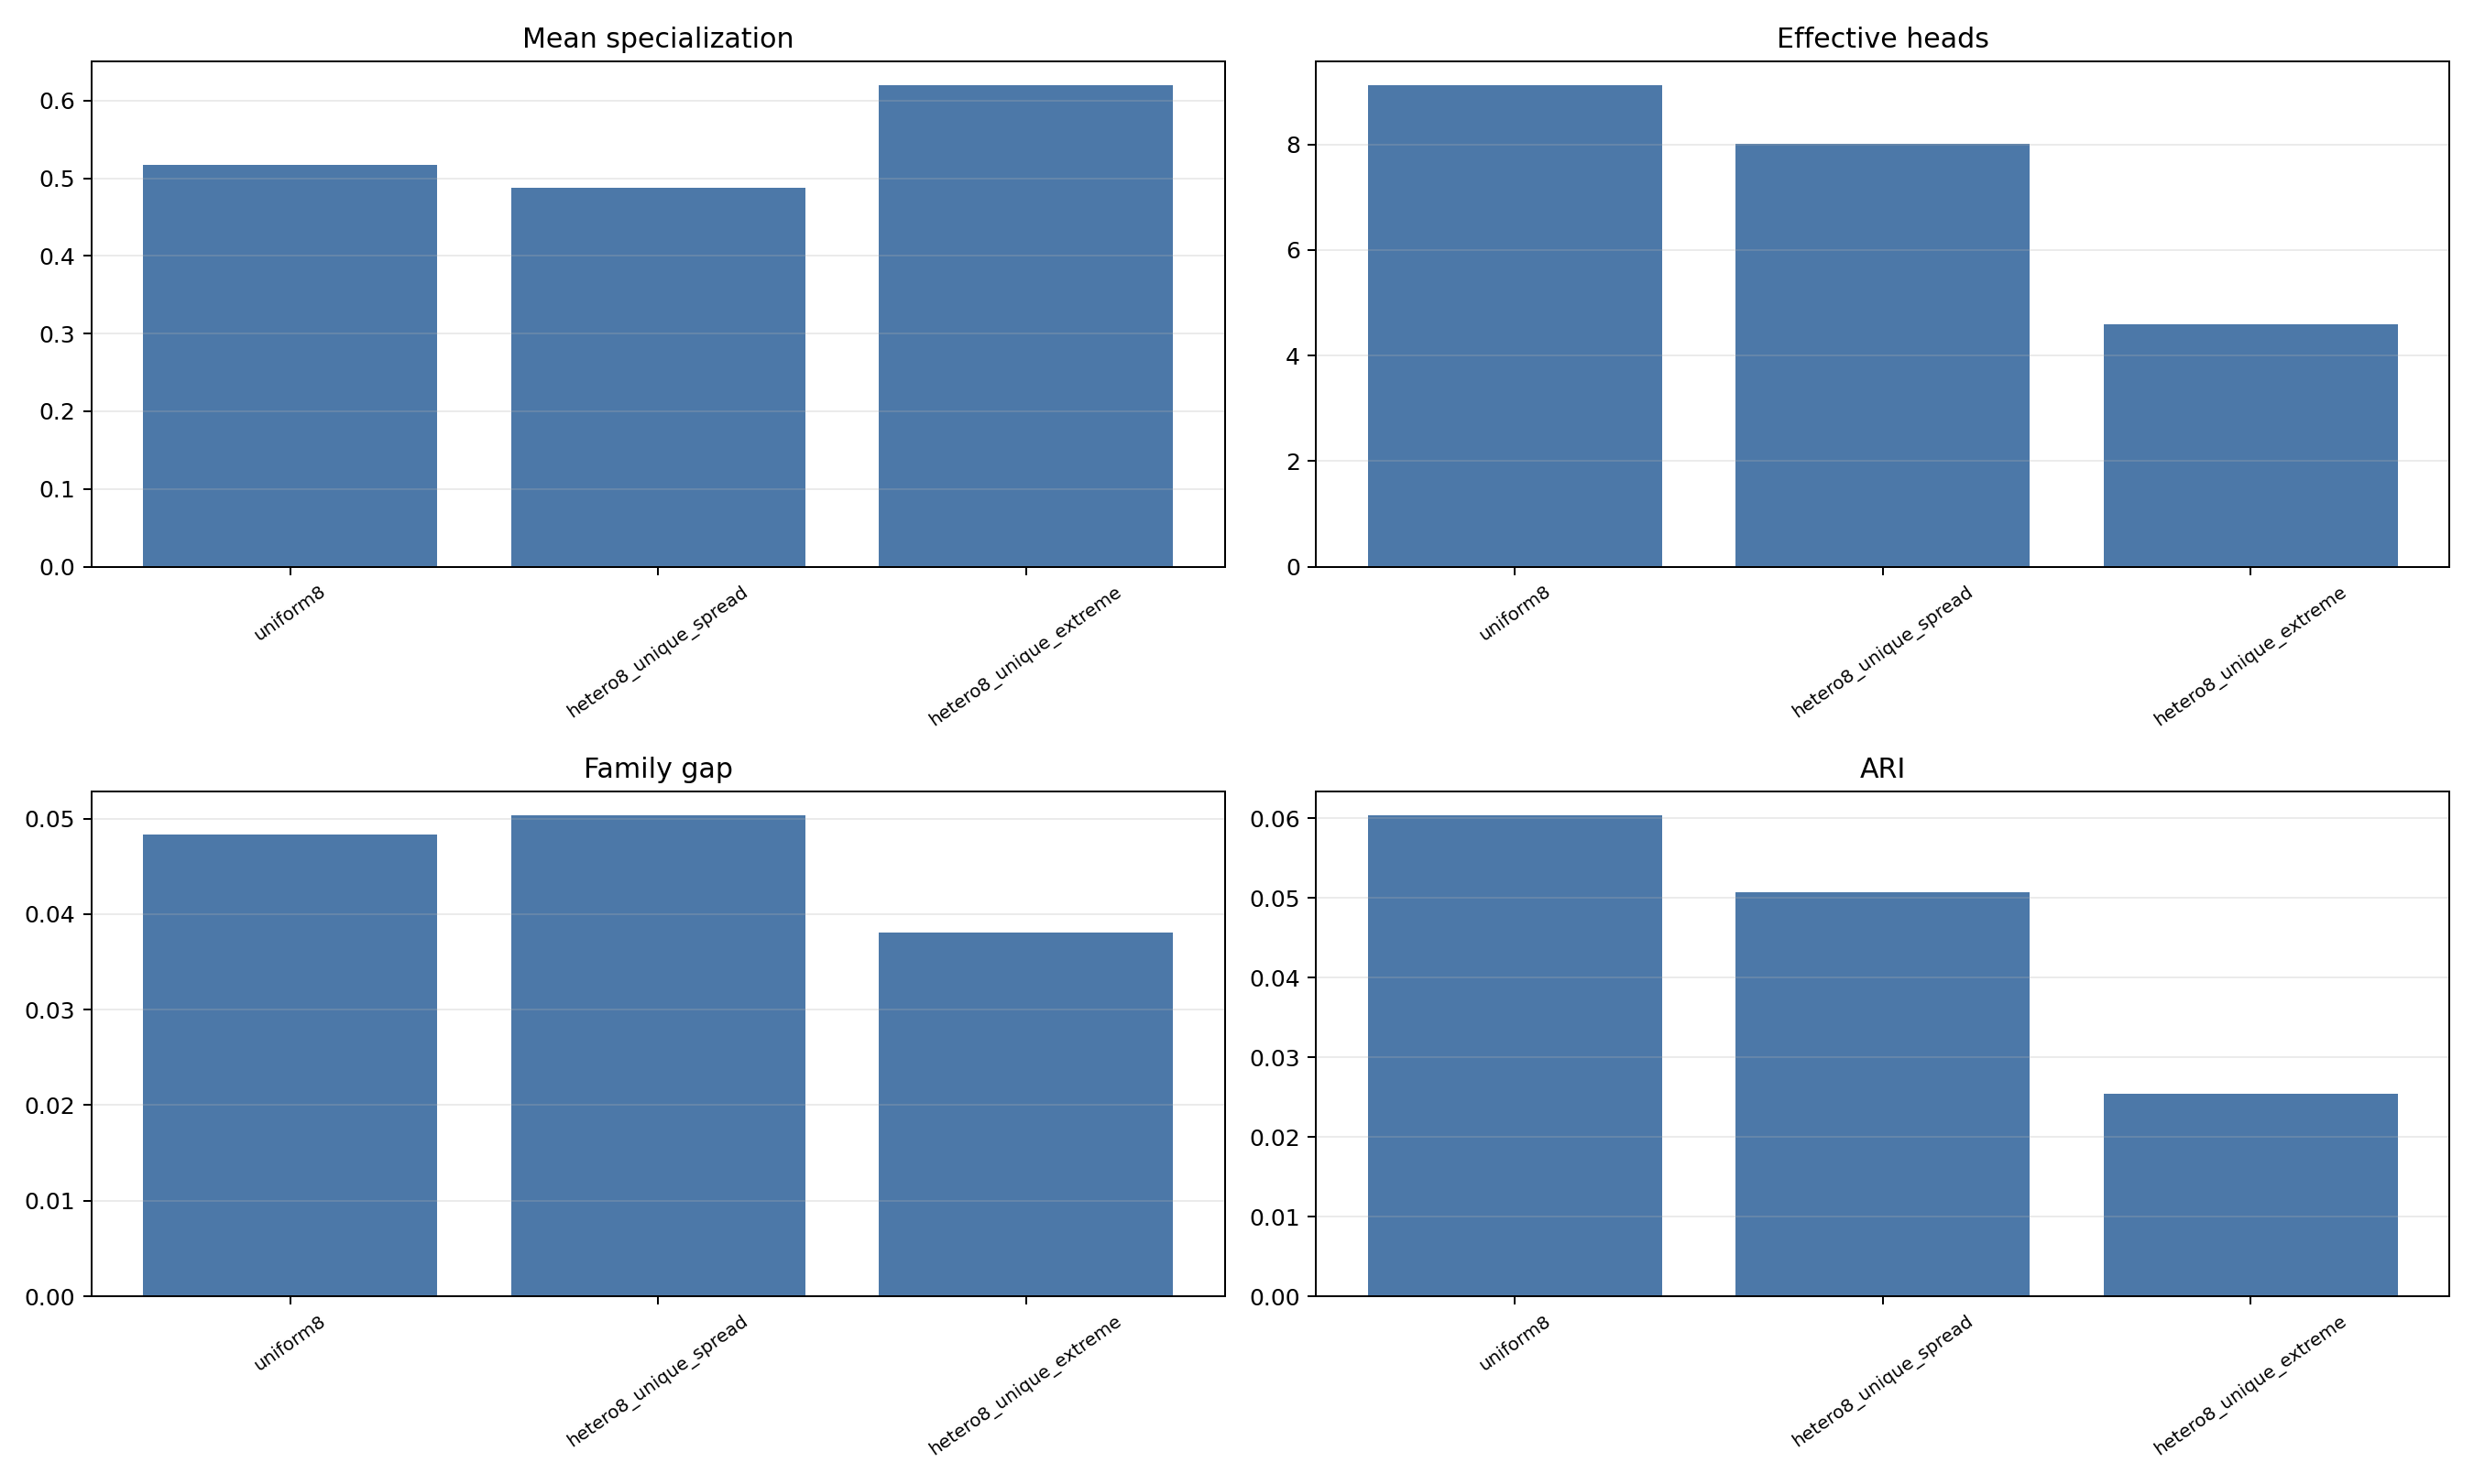
\includegraphics[width=0.90\linewidth]{../figures/large32_config_metric_bars.png}
\end{frame}

\begin{frame}{16-Slot Control}
  \small
  The first 1000-step 16-slot run undertrained \texttt{uniform8}.

  \vspace{0.25cm}
  Targeted fix:
  \begin{itemize}
    \item rerun the same 16-slot grid for 2000 steps;
    \item use the 2000-step run as the clean comparison.
  \end{itemize}
\end{frame}

\begin{frame}{16-Slot Clean Result}
  \scriptsize
  \begin{tabular}{lcccccc}
    \toprule
    Config & Min acc & Largest top & Spec & Eff heads & Gap & ARI \\
    \midrule
    \texttt{uniform8} & 0.978 & n/a & 0.514 & 5.314 & 0.132 & 0.130 \\
    \texttt{hetero8\_spread} & 0.988 & 0.62 & 0.609 & 3.923 & 0.079 & 0.046 \\
    \texttt{hetero8\_extreme} & 0.997 & 0.76 & 0.784 & 2.247 & 0.081 & 0.058 \\
    \bottomrule
  \end{tabular}

  \vspace{0.35cm}
  Interpretation: hetero improves specialization but does not beat the uniform8 baseline on family modularity.
\end{frame}

\begin{frame}{16-Slot Plot}
  \centering
  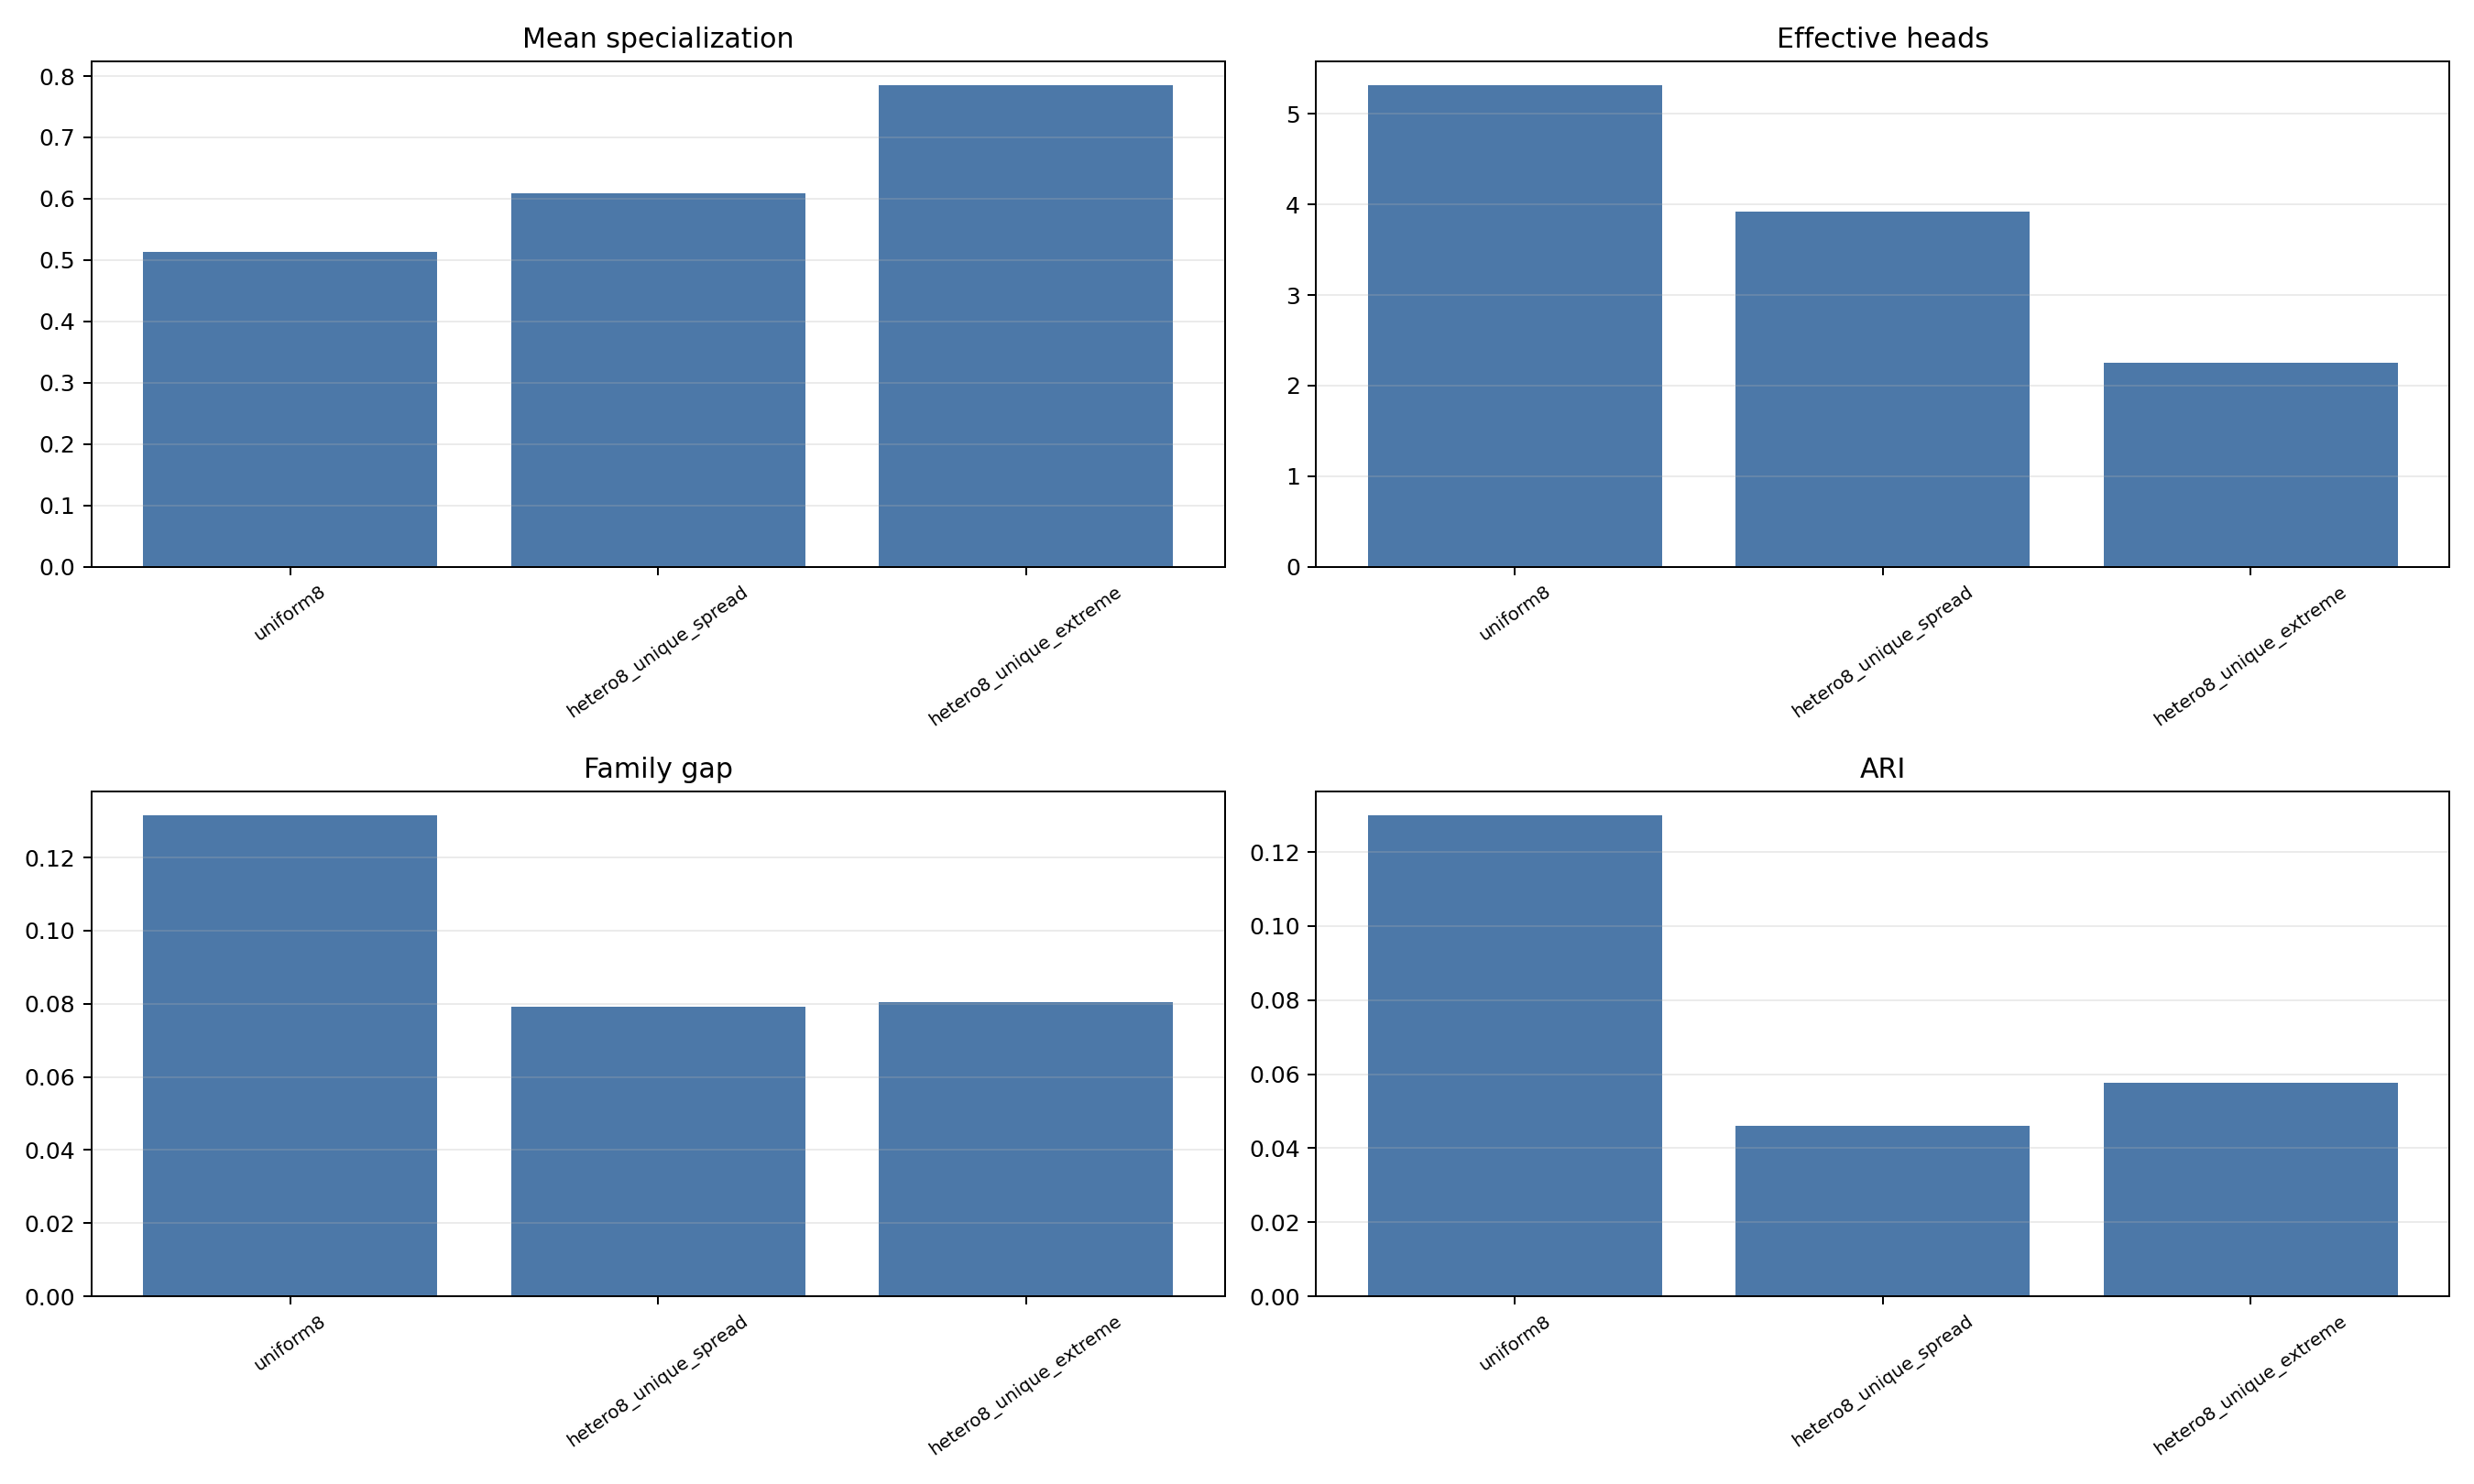
\includegraphics[width=0.90\linewidth]{../figures/large16_config_metric_bars.png}
\end{frame}

\begin{frame}{Answer To The Head-Count Concern}
  \large
  More heads do not rescue the modularity claim.

  \vspace{0.4cm}
  \normalsize
  They preserve the stronger results:
  \begin{itemize}
    \item structural role affinity remains far above chance;
    \item role-level specialization increases under stronger heterogeneity;
    \item family-level modularity remains separate and not automatic.
  \end{itemize}
\end{frame}

\begin{frame}{Failure Analysis}
  \scriptsize
  \begin{tabular}{p{0.35\linewidth}p{0.47\linewidth}}
    \toprule
    Possible factor & Evidence \\
    \midrule
    Too few heads & Less likely after 16-slot and 32-slot controls. \\
    Too much depth fragments exact slots & 32-slot gap is weaker than 16-slot gap. \\
    Role difficulty, not family, drives large-head choice & Many unrelated roles go to the largest head. \\
    Ontology family labels are too coarse & Induction and boundary subroles behave differently inside family. \\
    Extreme imbalance causes collapse & Extreme configs specialize strongly but have weak ARI. \\
    \bottomrule
  \end{tabular}
\end{frame}

\begin{frame}{Real-Model Probe}
  \small
  Pythia-160M-deduped, revision \texttt{step143000}, ordinary attention heads.

  \vspace{0.25cm}
  The first float16 run produced NaNs in later-layer attention summaries.
  The float32 rerun had no NaN rows and is the one reported here.
\end{frame}

\begin{frame}{Pythia Attention Role Results}
  \scriptsize
  \begin{tabular}{lccccc}
    \toprule
    Role & Best layer & Best head & Top spec & Eff heads & Interpretation \\
    \midrule
    \texttt{repeat\_match} & 0 & 7 & 0.834 & 2.088 & strong repeat/induction-like role \\
    \texttt{repeat\_match} & 6 & 10 & 0.725 & 3.445 & second strong repeat layer \\
    \texttt{previous\_token} & 10 & 9 & 0.332 & 9.169 & measurable but distributed \\
    \texttt{bos} & 8 & 6 & 0.140 & 9.809 & diffuse sink behavior \\
    \bottomrule
  \end{tabular}
\end{frame}

\begin{frame}{Existing Causal Pythia Results}
  \scriptsize
  \begin{tabular}{lccccc}
    \toprule
    Probe & Own top & Random & Excess & Aligned & Same-index \\
    \midrule
    Local copy & 2.519 & 0.229 & 2.290 & 2.271 & 0.488 \\
    Natural repeat 8-gram & 0.387 & 0.016 & 0.372 & 0.315 & 0.033 \\
    \bottomrule
  \end{tabular}

  \vspace{0.35cm}
  Values are loss deltas from ordinary-head ablations in Pythia-160M seed runs.
\end{frame}

\begin{frame}{Interpretation}
  \small
  \begin{itemize}
    \item Real ordinary heads clearly support local-copy and repeat/induction roles.
    \item The real-model evidence validates the role-measurement side of the project.
    \item It does not test heterogeneous dimensions, because Pythia heads are uniform.
    \item The current paper claim should separate structural affinity, specialization, and modularity.
  \end{itemize}
\end{frame}

\begin{frame}{Current Best Claim}
  \begin{quote}
    Heterogeneous ordinary attention-head dimensions create structural role affinity and usually increase role-level specialization.
  \end{quote}

  \vspace{0.35cm}
  \begin{quote}
    Larger-head controls do not show that heterogeneity automatically improves family-level modularity.
  \end{quote}
\end{frame}

\begin{frame}{Next Step}
  \small
  \begin{enumerate}
    \item Keep the larger-head result as a negative/moderating result for modularity.
    \item Add role-difficulty analysis: sequence distance, conflict, target entropy, and largest-head preference.
    \item Expand weak ontology families: induction, boundary/sink, suppression/conflict.
    \item Continue real ordinary-head causal probes for repeat, local copy, copy suppression, and IOI.
    \item Do not claim full functional modularity unless hetero beats matched uniform baselines.
  \end{enumerate}
\end{frame}

\begin{frame}[fragile]{Provenance}
  \tiny
  \begin{verbatim}
doc/experiments/phase3/phase3_large_head_count_and_real_validation.md
results/phase3_toy_role_ontology_v2_large_heads_1000_20260523
results/phase3_toy_role_ontology_v2_large_heads_2layer_2000_20260523
results/phase3_real_model_role_probe_pythia160m_deduped_float32_20260524
results/phase1_pythia160m_local_copy_candidate_pool_layers2_4_top2
results/phase1_pythia160m_wikitext103_natural_repeat_8gram_task_alignment_seed9_n128
  \end{verbatim}
\end{frame}

\end{document}
